%-----------------------------------------------
% Template para criação de resumos de projectos/dissertação
% jlopes AT fe.up.pt,   Fri Jul  3 11:08:59 2009
%-----------------------------------------------

\documentclass[9pt,a4paper]{extarticle}

%% English version: comment first, uncomment second
%\usepackage[portuguese]{babel}  % Portuguese
\usepackage[english]{babel}     % English
\usepackage{graphicx}           % images .png or .pdf w/ pdflatex OR .eps w/ latex
\usepackage{times}              % use Times type-1 fonts
\usepackage[utf8]{inputenc}     % 8 bits using UTF-8
\usepackage{url}                % URLs
\usepackage{multicol}           % twocolumn, etc
\usepackage{float}              % improve figures & tables floating
\usepackage[tableposition=top]{caption} % captions
%% English version: comment first (maybe)
\usepackage{indentfirst}        % portuguese standard for paragraphs
%\usepackage{parskip}

%% page layout
\usepackage[a4paper,margin=30mm,noheadfoot]{geometry}

%% space between columns
\columnsep 12mm

%% headers & footers
\pagestyle{empty}

%% figure & table caption
\captionsetup{figurename=Fig.,tablename=Tab.,labelsep=endash,font=bf,skip=.5\baselineskip}

%% heading
\makeatletter
\renewcommand*{\@seccntformat}[1]{%
  \csname the#1\endcsname.\quad
}
\makeatother

%% avoid widows and orphans
\clubpenalty=300
\widowpenalty=300

\begin{document}

\title{\vspace*{-8mm}\textbf{\textsc{Improving Variability of Applications using Adaptive Object-Models}}}
\author{\emph{João Gradim Pereira}\\[2mm]
\small{Dissertation realized under the supervision of \emph{Ademar Aguiar (Ph.D.)} and \emph{Hugo Ferreira (Ph.D. AbD)}}\\
\small{at \emph{Tecla Colorida, Lda}}}
\date{}
\maketitle
%no page number 
\thispagestyle{empty}

\vspace*{-4mm}\noindent\rule{\textwidth}{0.4pt}\vspace*{4mm}

\begin{multicols}{2}

\section{Motivation}\label{sec:motivation}

%Software systems are usually designed with a specific purpose in mind. They rely on a series of requirements which are often very difficult to capture and maintain, as they have a tendency to evolve faster than the implementation. This is caused mainly by the poor understanding by the stakeholders about their needs and expectations about what a software system should be able to do~\cite{PT07}. These situations lead to higher costs in software development, as creating and maintaining software systems is a knowledge intensive task~\cite{AdOdSBD07}. Moreover, most of these system are not static, and have a constant need to evolve in order to adapt themselves to their environment and new business rules, shifting the stakeholders' needs and expectations about these software systems.
Software systems are usually designed with a specific purpose in mind. They rely on a series of requirements which are often very difficult to capture and maintain, as they have a tendency to evolve faster than the implementation. This is caused mainly by the poor understanding by the stakeholders about their needs and expectations about what a software system should be able to do. These situations lead to higher costs in software development, as creating and maintaining software systems is a knowledge intensive task. Moreover, most of these system are not static, and have a constant need to evolve in order to adapt themselves to their environment and new business rules, shifting the stakeholders' needs and expectations about these software systems.

%In face of these situations, new development methods started to focus more on iterative and incremental approaches, accepting \emph{incompleteness} as part of every software system's development cycle~\cite{WC03}. At the same time, many new systems are being developed with an emphasis on flexibility and run-time configuration~\cite{YJ02}.
In face of these situations, new development methods started to focus more on iterative and incremental approaches, accepting \emph{incompleteness} as part of every software system's development cycle. At the same time, many new systems are being developed with an emphasis on flexibility and run-time configuration~\cite{YJ02}.

\section{Objectives}\label{sec:objectives}

At the same time, many new systems are being developed with an emphasis on flexibility and run-time configuration~\cite{YJ02}. An Adaptive Object-Model (AOM) is an architectural style based on metamodeling and object-oriented design that exposes its domain model to the end-user, and aims to create better mechanisms for the evolution and adaption of software systems to their environments.

The first chalenge is to adapt some of the ideologies and techniques of the AOM architectural style to a Ruby on Rails application (using an MVC architecture), using an application design based on a static schema from a relational database (MySQL), by applying a series of design patterns connected with AOM architectures. Three areas within the \emph{escolinhas.pt} platform were chosen to perform this refactoring: User Roles, Social Network and Document Editor.

The second goal is to measure how the variability and performance of each component are affected by the application of these design patterns.

\section{User Roles}\label{sec:user_roles}

In \emph{escolinhas.pt}, user roles are organized as an \textsc{Organization Hierarchy}~\cite{fowler_accountability}. This creates some problems when trying to create new roles or give special privileges to an user, due to multi-level hierarchy used.

%\begin{figure}[H]
%  \centering{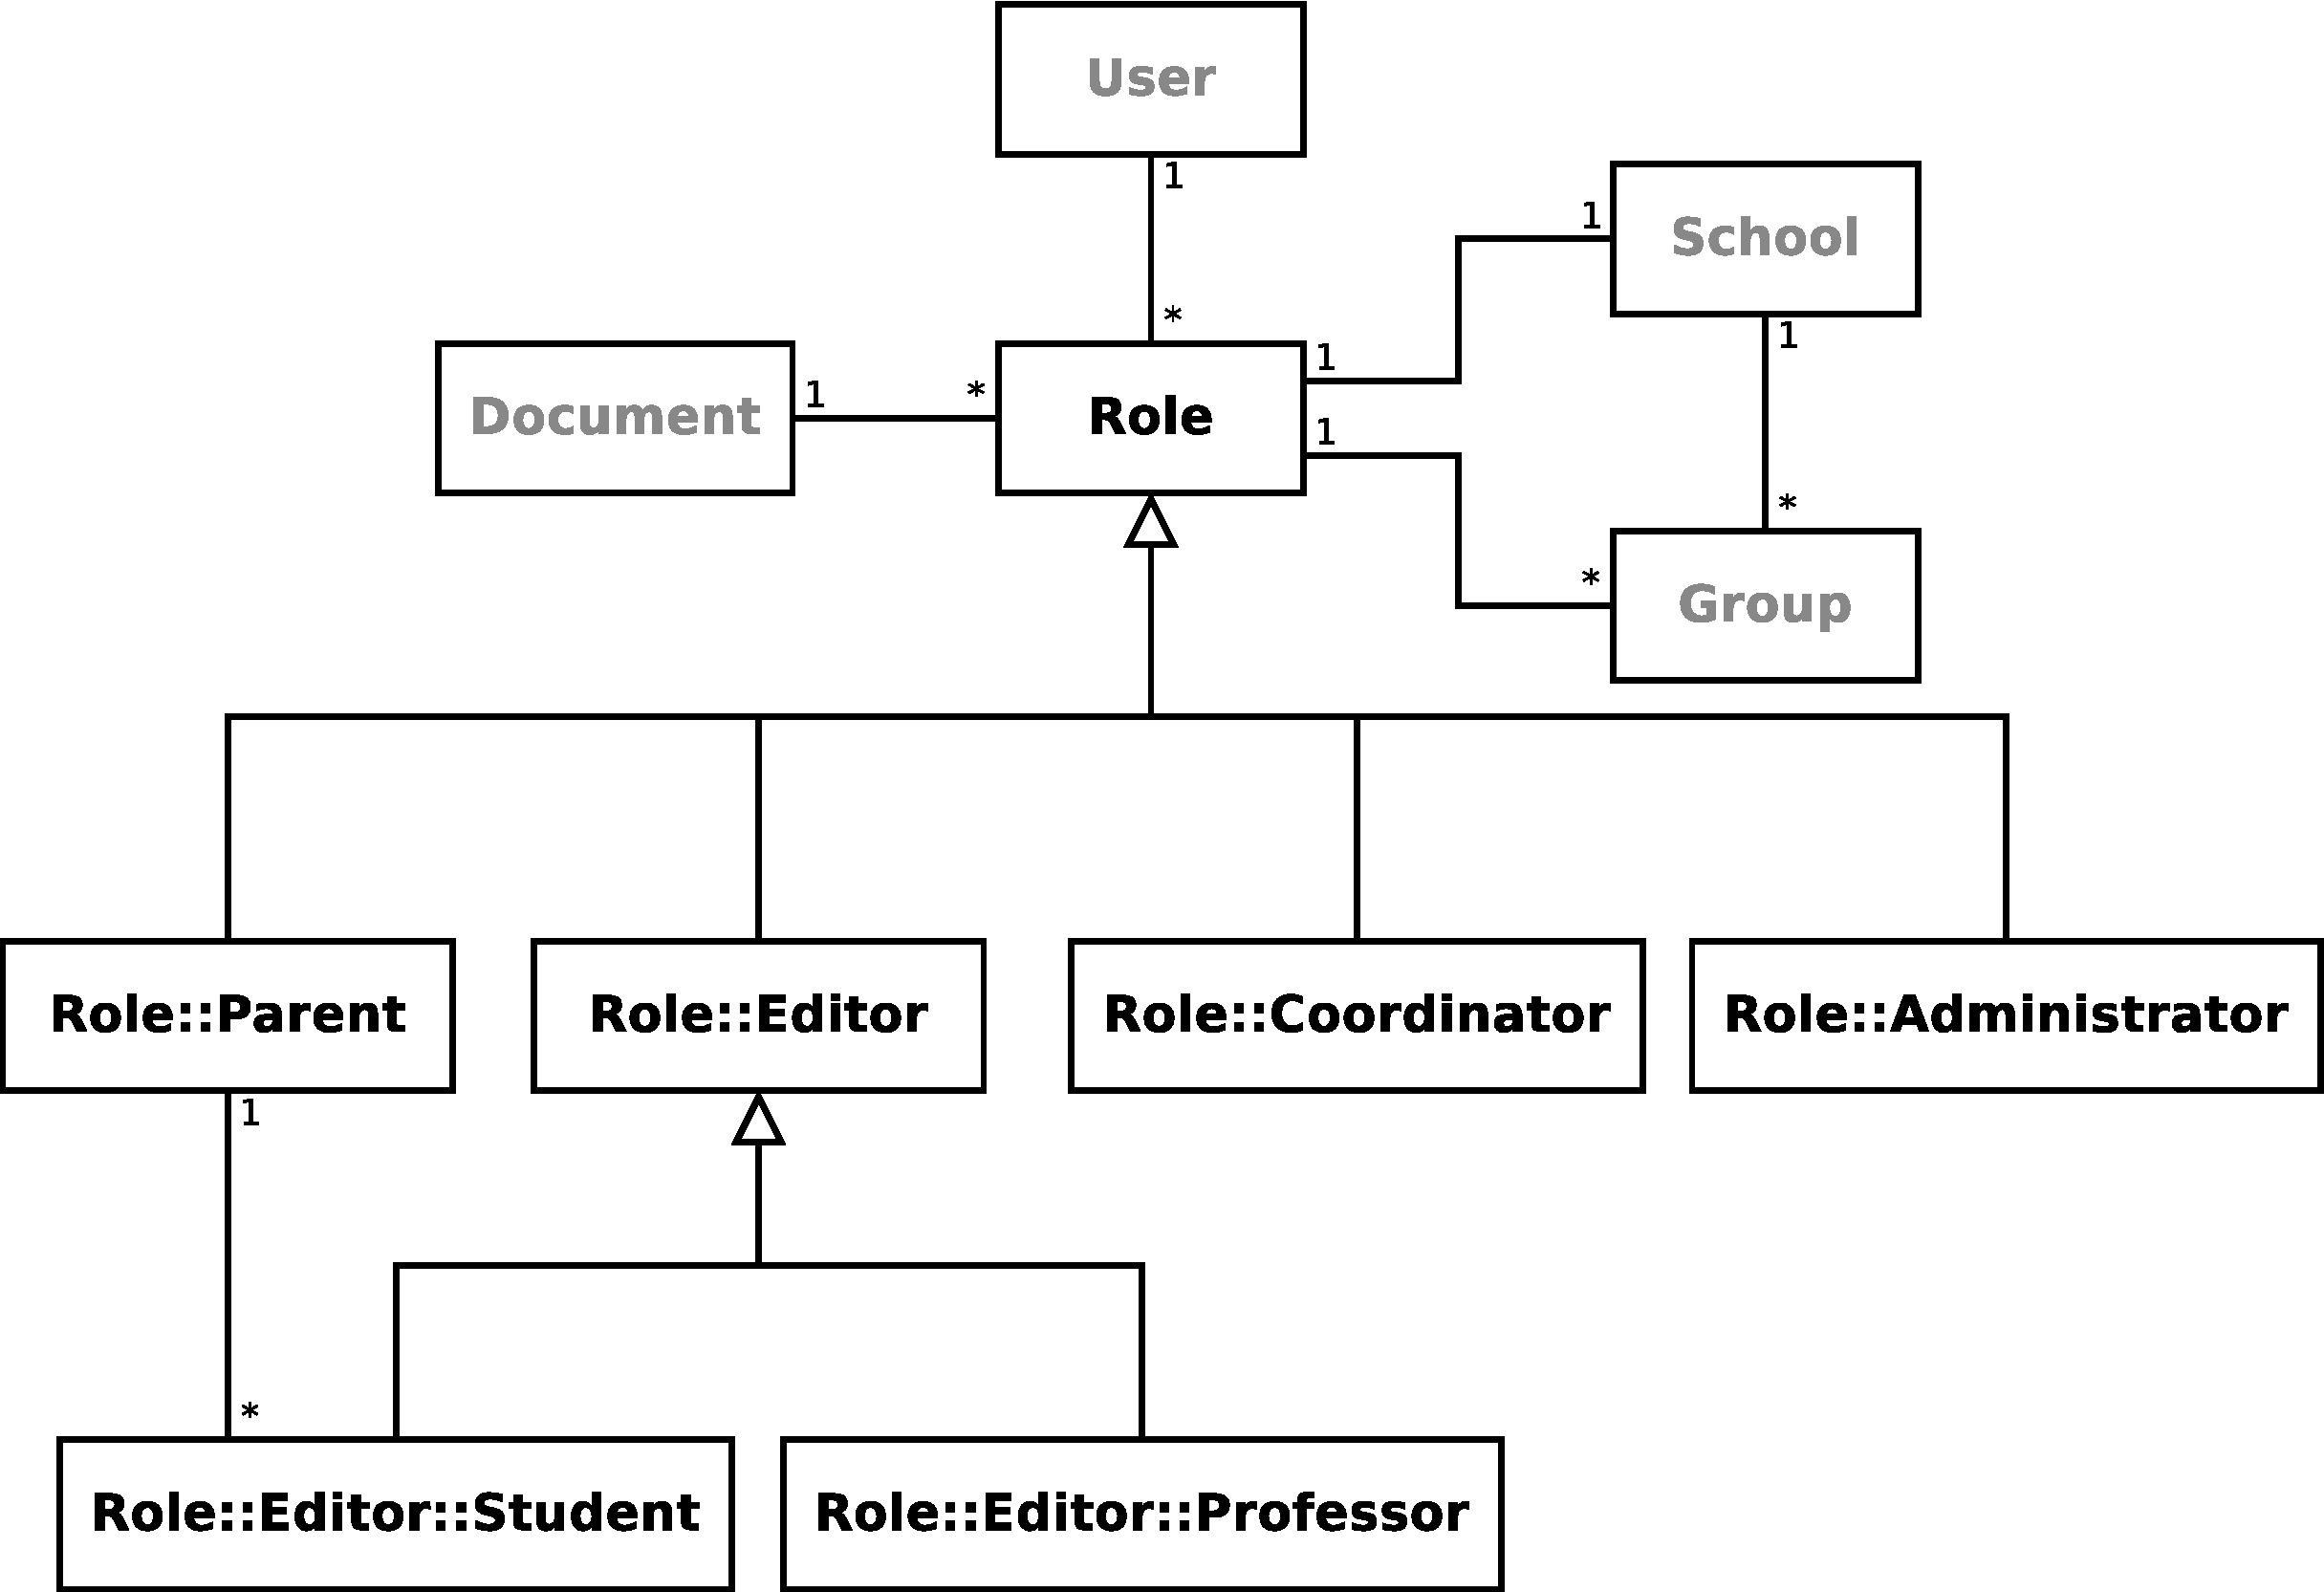
\includegraphics[width=0.4\textwidth]{figures/user_roles_current}}
%  \caption{sasdasd}
%  \label{fig:user_roles_current}
%\end{figure}

By using the \textsc{Role Object} pattern, the roles are split into single classes, which allows capturing the key abstractions of each one individually. By discarding the hierarchy present before and transforming

%\begin{figure}[H]
%  \centering{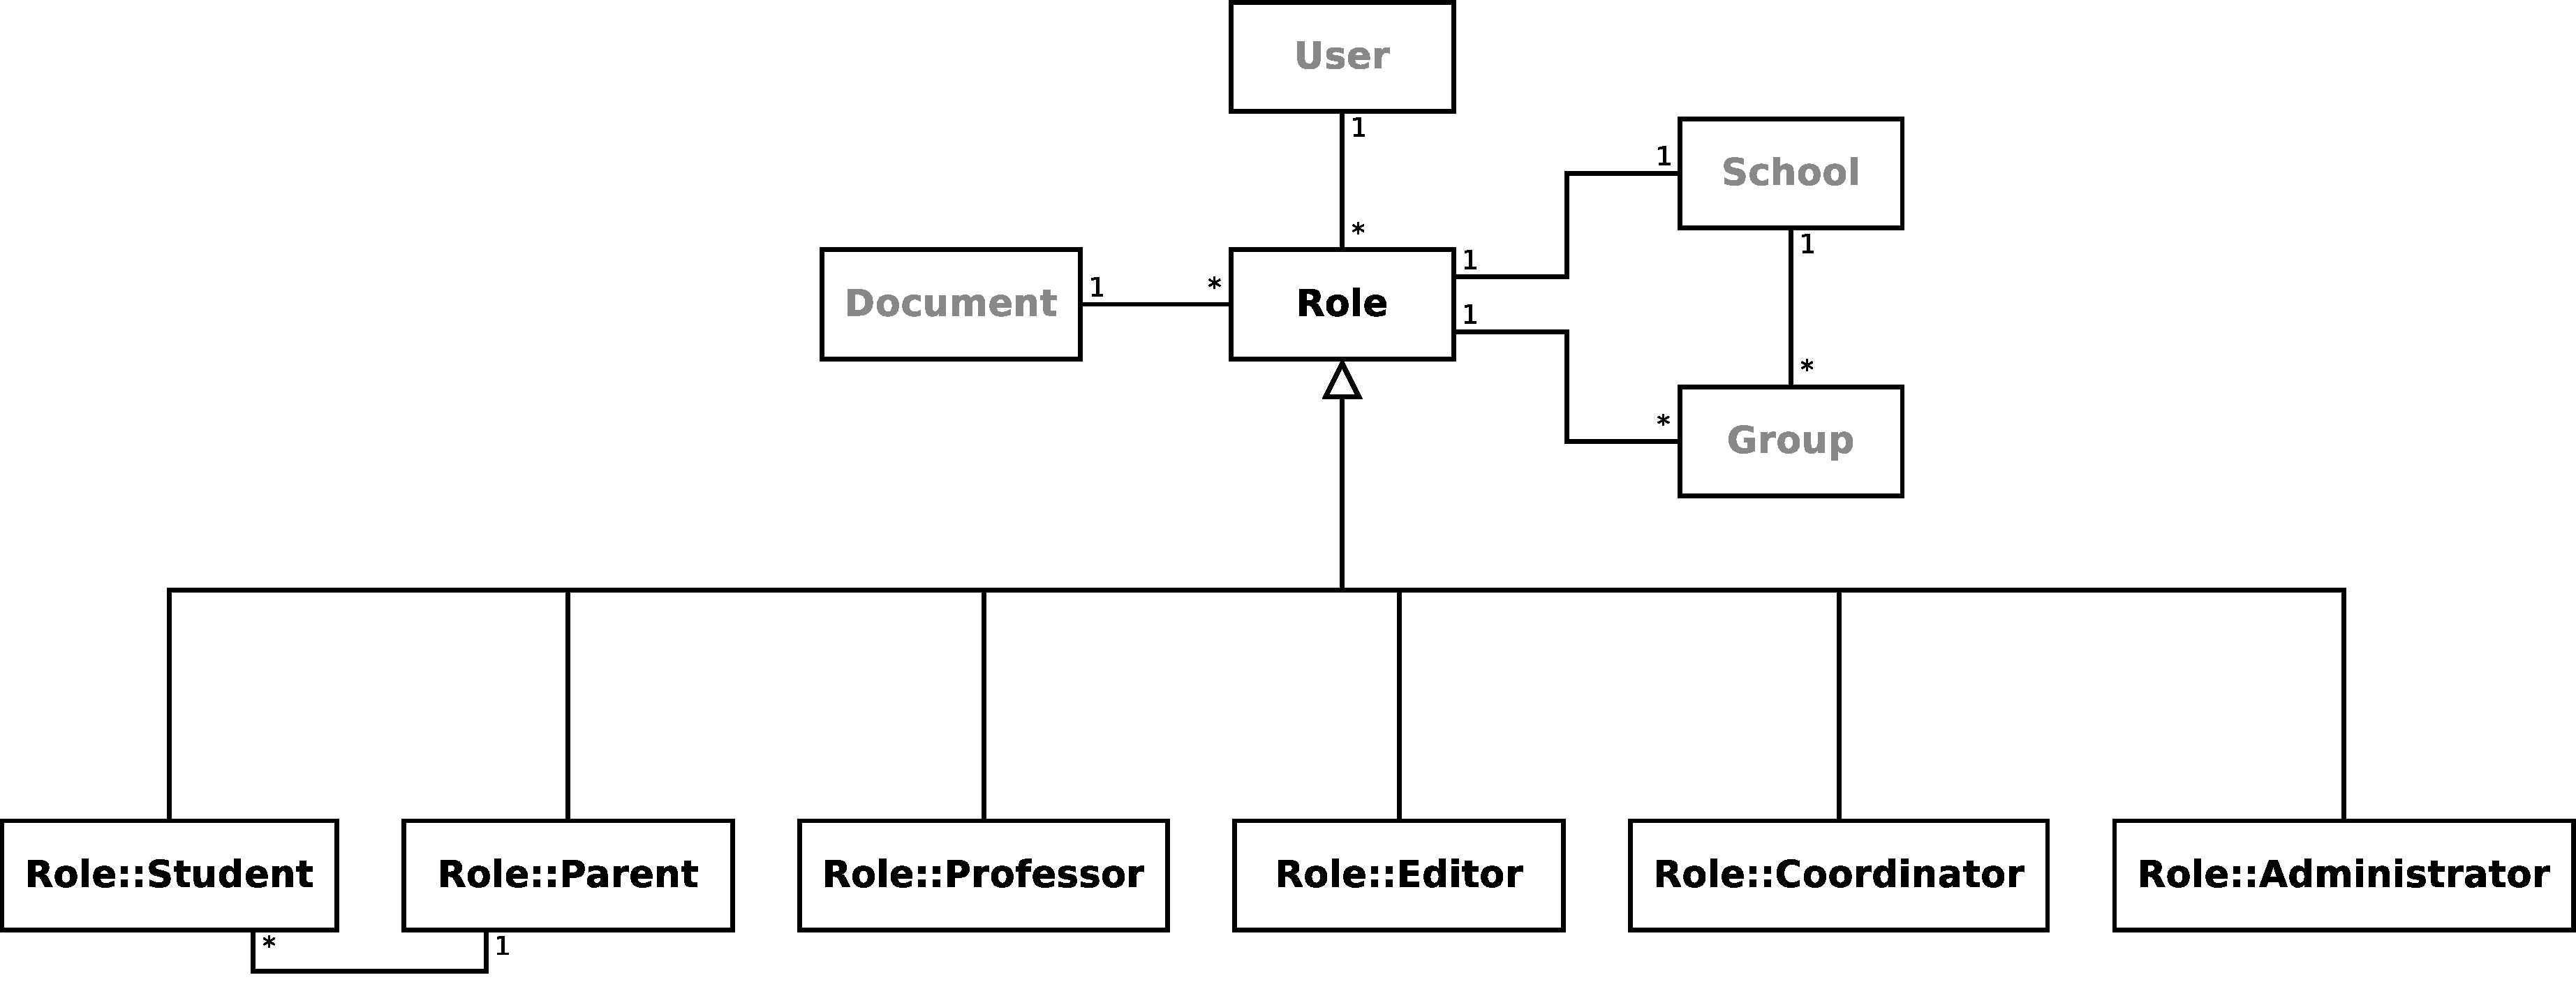
\includegraphics[width=0.4\textwidth]{figures/user_roles_conceptual}}
%  \caption{sasdasd}
%  \label{fig:user_roles_conceptual}
%\end{figure}

\section{Social Network}\label{sec:social_network}

The current design for the escolinhas.pt social network is based on the relationships formed through the connections between users and their schools, groups, and other users, as depicted in Fig.~\ref{fig:social_network_current}. This allows the construction of a network where all the connections can be inferred dynamically and where an user can be identified towards another through these same connections. This model, however useful, offers a very small degree of variability.

\begin{figure}[H]
  \centering{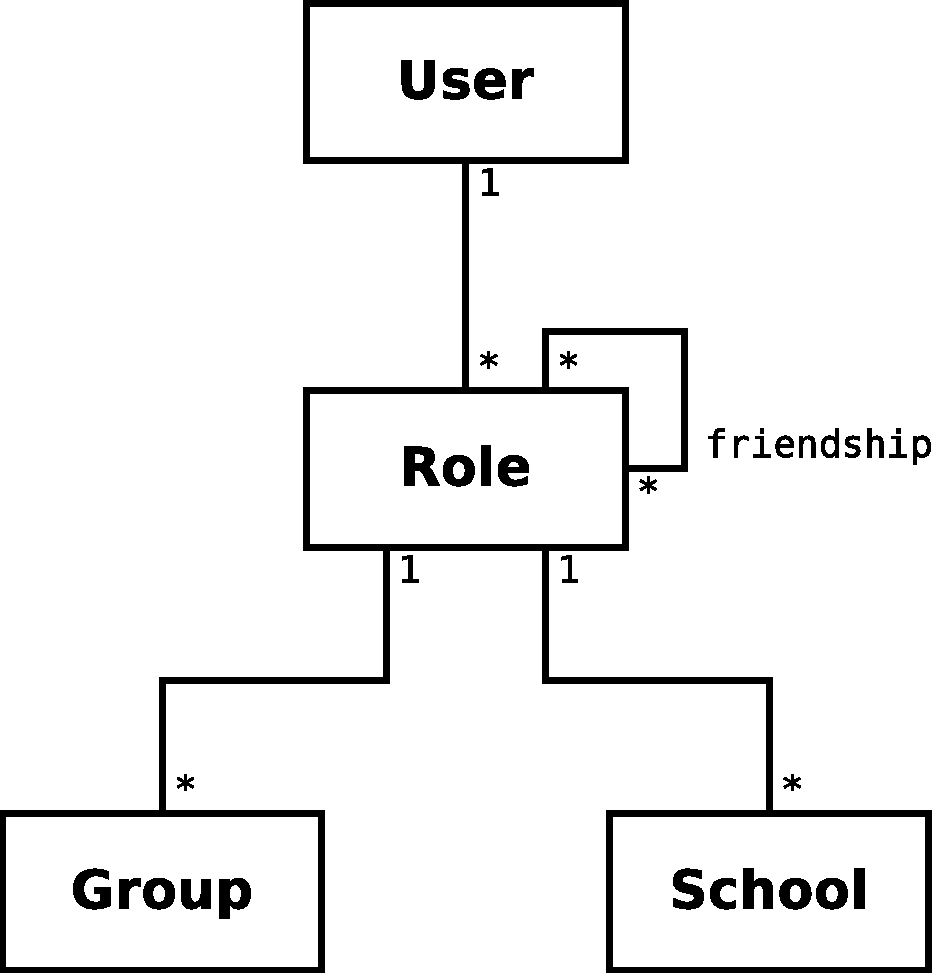
\includegraphics[width=35mm]{figures/social_network_current}}
  \caption{sasdasd}
  \label{fig:social_network_current}
\end{figure}

The usage of the \textsc{Accountability} design pattern, by Martin Fowler~\cite{fowler_accountability} allows the creation of a relationship between two different entities in the system, with a third optional entity providing more information as to how they are connected.

\begin{figure}[H]
  \centering{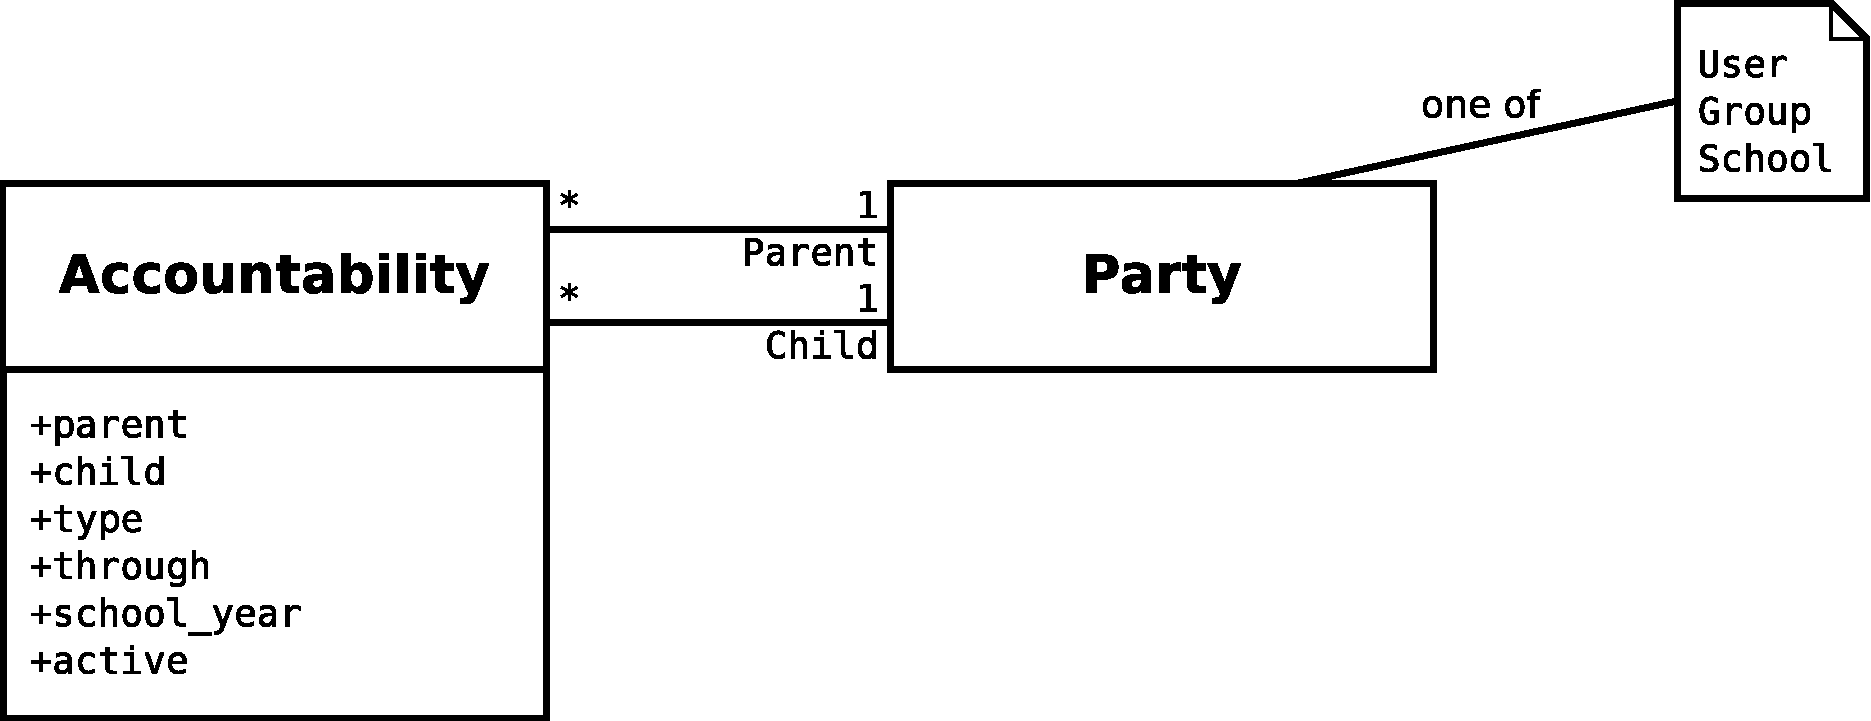
\includegraphics[width=0.4\textwidth]{figures/social_network_conceptual}}
  \caption{sasdasd}
  \label{fig:social_network_conceptual}
\end{figure}

\section{Document Editor}\label{sec:document_editor}

The document editor present in \emph{escolinhas.pt} is one of the core components of the system and one of the used features of the platform. This being the case, and due to the constantly evolving nature of the product and the product itself, it is also one of the most modified parts of the system. The document editor infrastructure has to grow both in size and complexity every time a new type of block content is introduced --- represented by the gray entities in Fig.~\ref{fig:documents_current} --- by creating 

\begin{figure}[H]
  \centering{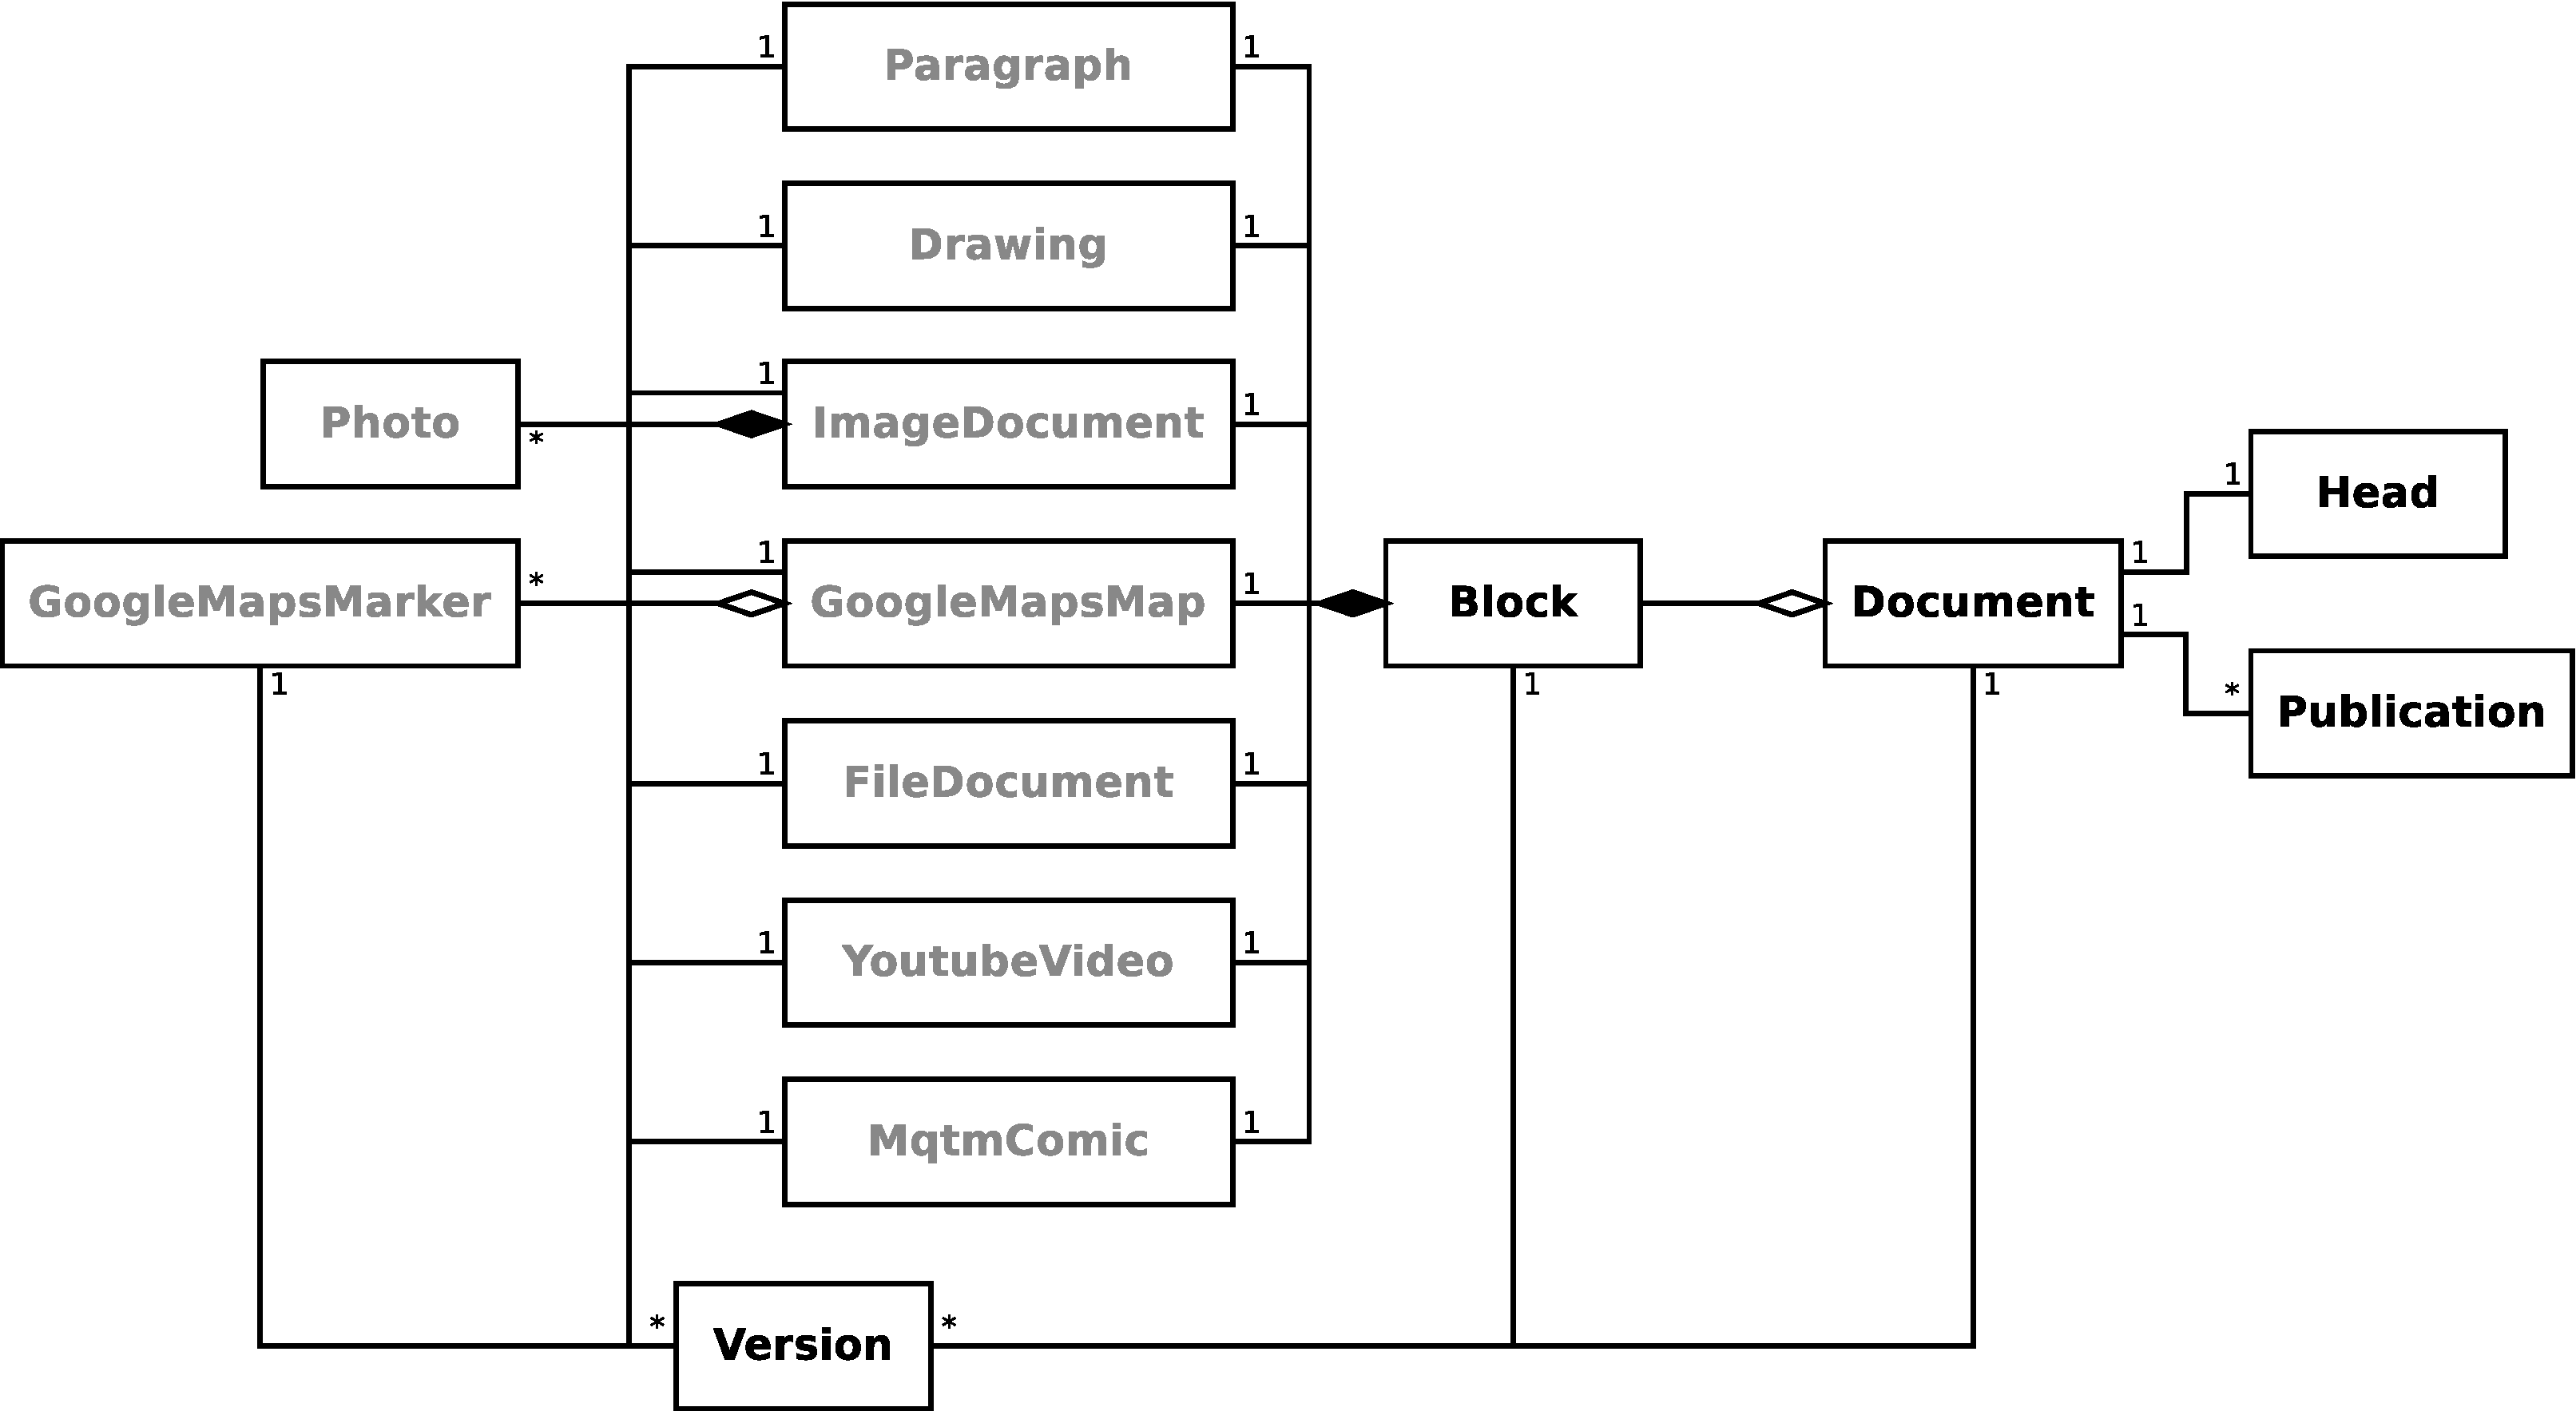
\includegraphics[width=0.4\textwidth]{figures/documents_current}}
  \caption{sasdasd}
  \label{fig:documents_current}
\end{figure}

The solution devised for the \emph{Documents} infrastructure is, the simplest structure possible that makes everything work (as seen in Fig.~\ref{fig:documents_conceptual}). This is made possible by using a variant of the \textsc{Property} pattern~\cite{metadata_and_active_object_models} and the \textsc{System Memento}~\cite{patterns_data_and_metadata_evolution_in_aoms}

\begin{figure}[H]
  \centering{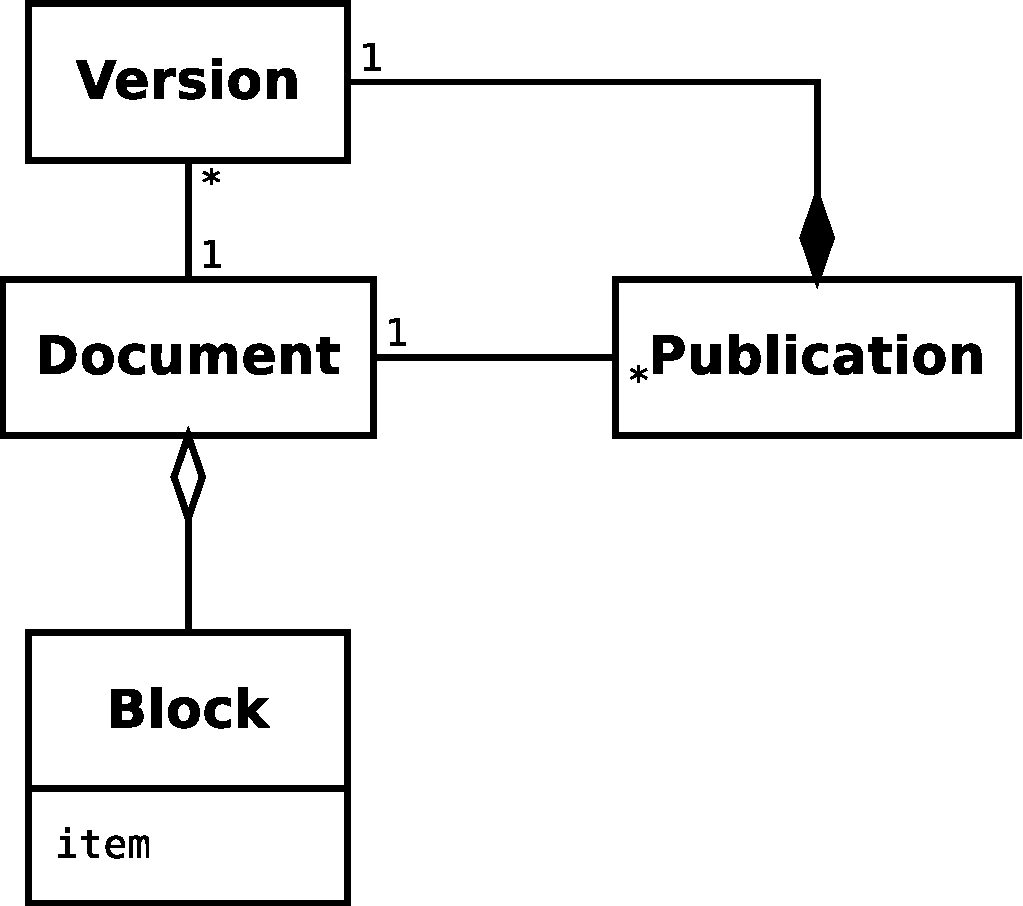
\includegraphics[width=25mm]{figures/documents_conceptual}}
  \caption{sasdasd}
  \label{fig:documents_conceptual}
\end{figure}

\section{Conclusion}\label{sec:conclusion}

Despite being built with a MVC architecture, the Ruby On Rails framework is, using the right approach, capable of working with some architectural and design patterns --- present in AOM architectures --- not obviously connected with MVC and AR. The application of these patterns is capable of increasing the level of variability present in a common Rails application, and a harmonious integration with the Rails 2.3.x infrastructure --- especially the \textsc{ActiveRecord} engine --- is possible and works elegantly.

It is also possible to conclude that the application of the appropriate design patterns is able to increase not only the variability and configurability needs of a specific part of an application, but also its performance, in some cases. However, this should not be taken as an universal truth, as it depends on a series of factors that may not be present in all implementations, such as a previous innapropriate design.

%%English version: comment first, uncomment second
\bibliographystyle{unsrt-pt}  % numeric, unsorted refs
%\bibliographystyle{numeric}  % numeric, unsorted refs
\bibliography{article-en}

\end{multicols}

\end{document}
